%%%%%%%%%%%%%%%%%%%%%%%%%%%%%%%%%%%%%%%%%%%%%%%%%%%%%%%%%%%%%%%%%%%%%
%% This is a (brief) model paper using the achemso class
%% The document class accepts keyval options, which should include
%% the target journal and optionally the manuscript type. 
%%%%%%%%%%%%%%%%%%%%%%%%%%%%%%%%%%%%%%%%%%%%%%%%%%%%%%%%%%%%%%%%%%%%%
\documentclass[journal=jacsat,manuscript=article]{achemso}

%%%%%%%%%%%%%%%%%%%%%%%%%%%%%%%%%%%%%%%%%%%%%%%%%%%%%%%%%%%%%%%%%%%%%
%% Place any additional packages needed here.  Only include packages
%% which are essential, to avoid problems later. Do NOT use any
%% packages which require e-TeX (for example etoolbox): the e-TeX
%% extensions are not currently available on the ACS conversion
%% servers.
%%%%%%%%%%%%%%%%%%%%%%%%%%%%%%%%%%%%%%%%%%%%%%%%%%%%%%%%%%%%%%%%%%%%%
\usepackage[version=3]{mhchem} % Formula subscripts using \ce{}

%%%%%%%%%%%%%%%%%%%%%%%%%%%%%%%%%%%%%%%%%%%%%%%%%%%%%%%%%%%%%%%%%%%%%
%% If issues arise when submitting your manuscript, you may want to
%% un-comment the next line.  This provides information on the
%% version of every file you have used.
%%%%%%%%%%%%%%%%%%%%%%%%%%%%%%%%%%%%%%%%%%%%%%%%%%%%%%%%%%%%%%%%%%%%%
%%\listfiles

%%%%%%%%%%%%%%%%%%%%%%%%%%%%%%%%%%%%%%%%%%%%%%%%%%%%%%%%%%%%%%%%%%%%%
%% Place any additional macros here.  Please use \newcommand* where
%% possible, and avoid layout-changing macros (which are not used
%% when typesetting).
%%%%%%%%%%%%%%%%%%%%%%%%%%%%%%%%%%%%%%%%%%%%%%%%%%%%%%%%%%%%%%%%%%%%%
\newcommand*\YE[1]{Ye: \texttt{\textbf{#1}}}

%%\newcommand{\YE}[1]{\textcolor{blue}{#1}}

%%%%%%%%%%%%%%%%%%%%%%%%%%%%%%%%%%%%%%%%%%%%%%%%%%%%%%%%%%%%%%%%%%%%%
%% Meta-data block
%% ---------------
%% Each author should be given as a separate \author command.
%%
%% Corresponding authors should have an e-mail given after the author
%% name as an \email command. Phone and fax numbers can be given
%% using \phone and \fax, respectively; this information is optional.
%%
%% The affiliation of authors is given after the authors; each
%% \affiliation command applies to all preceding authors not already
%% assigned an affiliation.
%%
%% The affiliation takes an option argument for the short name.  This
%% will typically be something like "University of Somewhere".
%%
%% The \altaffiliation macro should be used for new address, etc.
%% On the other hand, \alsoaffiliation is used on a per author basis
%% when authors are associated with multiple institutions.
%%%%%%%%%%%%%%%%%%%%%%%%%%%%%%%%%%%%%%%%%%%%%%%%%%%%%%%%%%%%%%%%%%%%%
\author{Ye Ding}
\affiliation{ATOMBEAT Inc.}
\email{dingy01@dp.tech}
\author{Hang Zheng}
\affiliation{ATOMBEAT Inc.}
\author{Xi Chen}
\affiliation{ATOMBEAT Inc.}
\author{Dongxu Pan}
\affiliation{ATOMBEAT Inc.}
\author{Xinyan Wang}
\affiliation{ATOMBEAT Inc.}

%%%%%%%%%%%%%%%%%%%%%%%%%%%%%%%%%%%%%%%%%%%%%%%%%%%%%%%%%%%%%%%%%%%%%
%% The document title should be given as usual. Some journals require
%% a running title from the author: this should be supplied as an
%% optional argument to \title.
%%%%%%%%%%%%%%%%%%%%%%%%%%%%%%%%%%%%%%%%%%%%%%%%%%%%%%%%%%%%%%%%%%%%%
\title[An \textsf{achemso} demo]
  {Improving binding free energy predictions with Swap Monte Carlo for water sampling}

%%%%%%%%%%%%%%%%%%%%%%%%%%%%%%%%%%%%%%%%%%%%%%%%%%%%%%%%%%%%%%%%%%%%%
%% Some journals require a list of abbreviations or keywords to be
%% supplied. These should be set up here, and will be printed after
%% the title and author information, if needed.
%%%%%%%%%%%%%%%%%%%%%%%%%%%%%%%%%%%%%%%%%%%%%%%%%%%%%%%%%%%%%%%%%%%%%
\abbreviations{Free Energy Perturbation, Binding Free Energy, Monte Carlo, Water Sampling, Molecular Dynamics}
\keywords{American Chemical Society, \LaTeX}

%%%%%%%%%%%%%%%%%%%%%%%%%%%%%%%%%%%%%%%%%%%%%%%%%%%%%%%%%%%%%%%%%%%%%
%% The manuscript does not need to include \maketitle, which is
%% executed automatically.
%%%%%%%%%%%%%%%%%%%%%%%%%%%%%%%%%%%%%%%%%%%%%%%%%%%%%%%%%%%%%%%%%%%%%
\begin{document}

%%%%%%%%%%%%%%%%%%%%%%%%%%%%%%%%%%%%%%%%%%%%%%%%%%%%%%%%%%%%%%%%%%%%%
%% The "tocentry" environment can be used to create an entry for the
%% graphical table of contents. It is given here as some journals
%% require that it is printed as part of the abstract page. It will
%% be automatically moved as appropriate.
%%%%%%%%%%%%%%%%%%%%%%%%%%%%%%%%%%%%%%%%%%%%%%%%%%%%%%%%%%%%%%%%%%%%%
%\begin{tocentry}

%Some journals require a graphical entry for the Table of Contents.
%This should be laid out ``print ready'' so that the sizing of the
%text is correct.

%Inside the \texttt{tocentry} environment, the font used is Helvetica
%8\,pt, as required by \emph{Journal of the American Chemical
%Society}.

%The surrounding frame is 9\,cm by 3.5\,cm, which is the maximum
%permitted for  \emph{Journal of the American Chemical Society}
%graphical table of content entries. The box will not resize if the
%content is too big: instead it will overflow the edge of the box.

%This box and the associated title will always be printed on a
%separate page at the end of the document.

%\end{tocentry}

%%%%%%%%%%%%%%%%%%%%%%%%%%%%%%%%%%%%%%%%%%%%%%%%%%%%%%%%%%%%%%%%%%%%%
%% The abstract environment will automatically gobble the contents
%% if an abstract is not used by the target journal.
%%%%%%%%%%%%%%%%%%%%%%%%%%%%%%%%%%%%%%%%%%%%%%%%%%%%%%%%%%%%%%%%%%%%%
\begin{abstract}
Water molecules within and around the binding cavity can significantly influence the binding affinity of ligands. 
Proper sampling of these water molecules ensures that their contributions to the free energy landscape are accurately accounted for. 
In the pursuit of more accurate binding free energy calculations, we have developed a novel Swap Monte Carlo (SwapMC) method specifically designed for cavity water sampling. 
The SwapMC method aims to enhance the sampling efficiency by facilitating the movement of water molecules in and out of the protein cavity, thereby ensuring a comprehensive exploration of water distributions. 
By leveraging GPU power to perform Monte Carlo moves for water molecules in parallel across multiple sites, and integrating SwapMC with NPT simulations within the Uni-FEP framework, 
we have observed significant improvements in the accuracy of relative binding free energy calculations, all while maintaining computational efficiency. 
Our results demonstrate that SwapMC achieves performance comparable to Grand Canonical Monte Carlo (GCMC) methods in water-related test cases, offering a robust and efficient alternative for addressing the challenges associated with cavity water sampling in computational chemistry. 
%Furthermore, we have extended the SwapMC scheme to sample the distribution of ions in DNA/RNA simulations, 
%broadening the applicability of this method to a wider range of biomolecular systems and enhancing the accuracy of ion-related free energy calculations.
\end{abstract}

%%%%%%%%%%%%%%%%%%%%%%%%%%%%%%%%%%%%%%%%%%%%%%%%%%%%%%%%%%%%%%%%%%%%%
%% Start the main part of the manuscript here.
%%%%%%%%%%%%%%%%%%%%%%%%%%%%%%%%%%%%%%%%%%%%%%%%%%%%%%%%%%%%%%%%%%%%%
\section{Introduction}
%%\YE{TO be completed.}

\section{Method}
\subsection{Workflow of the Swap Monte Carlo}
SwapMC was designed to exchange water molecules in and out of the protein cavity during FEP calculations, Fig.~\ref{fig:scheme} A.
Unlike the rectangler region that defined in Ben-Shalom's work~\cite{ben2021fast}, 
the cavity region in our protocol is represented by a spherical space that centered at the geometric center of the ligand coordinates, $R^{in}$ in Fig.~\ref{fig:scheme} B.
The radius is half the maximum intra-atomic distance within the ligands, plus an additional 0.3 nanometers for buffer.
All other areas of the simulation box are considered outside this spherical cavity and will be referred to $R^{out}$ space hereafter, Fig.~\ref{fig:scheme} B.
Thus, the SwapMC algorithm workflow consists of these steps:
\begin{enumerate}
  \item Randomly decide the exchange direction, ensuring an equal chance of moving water in or out of the cavity.
  \item A water molecule $i$ is chosen for deletion from the source region with the probability defined in Eq.~\ref{eq:selection_probability}. 
    Where $u_i$ represents the interaction energy of water molecule $i$ with other atoms in the simulation box. 
    $N_{src}$ denotes the number of exchangeable water molecules in the source region. A higher $u_i$ increases the likelihood of a molecule being selected.
  \begin{equation}\label{eq:selection_probability}
     p_i = \frac{e^{u_i}}{\sum^{N_{src}}_k{e^{u_k}}} \tag{1}    
  \end{equation}
  \item Uniform sampling the potential insertion sites over the destination region.
  \item The combination of the sampled sites with 60 orientations of water molecule results in 18,000 possible insertion conformations.
  \item Evaluate the interaction energy for each of the 18,000 water molecules in the simulated system, denoted as $u_j$.
  \item Sequentially iterate over the potential insertion confomation, and calculate the acceptance ratio $A_{S_i, S_j}$ using $u_i$ and $u_j$, determine if the conformation is acceptable. 
  If it is, terminate this iteration.
  \item Replace the deleted water positions by the accepted conformation coordinates and set this water molecule's velocity to zero for the simulation stability.
\end{enumerate}
\begin{figure}
  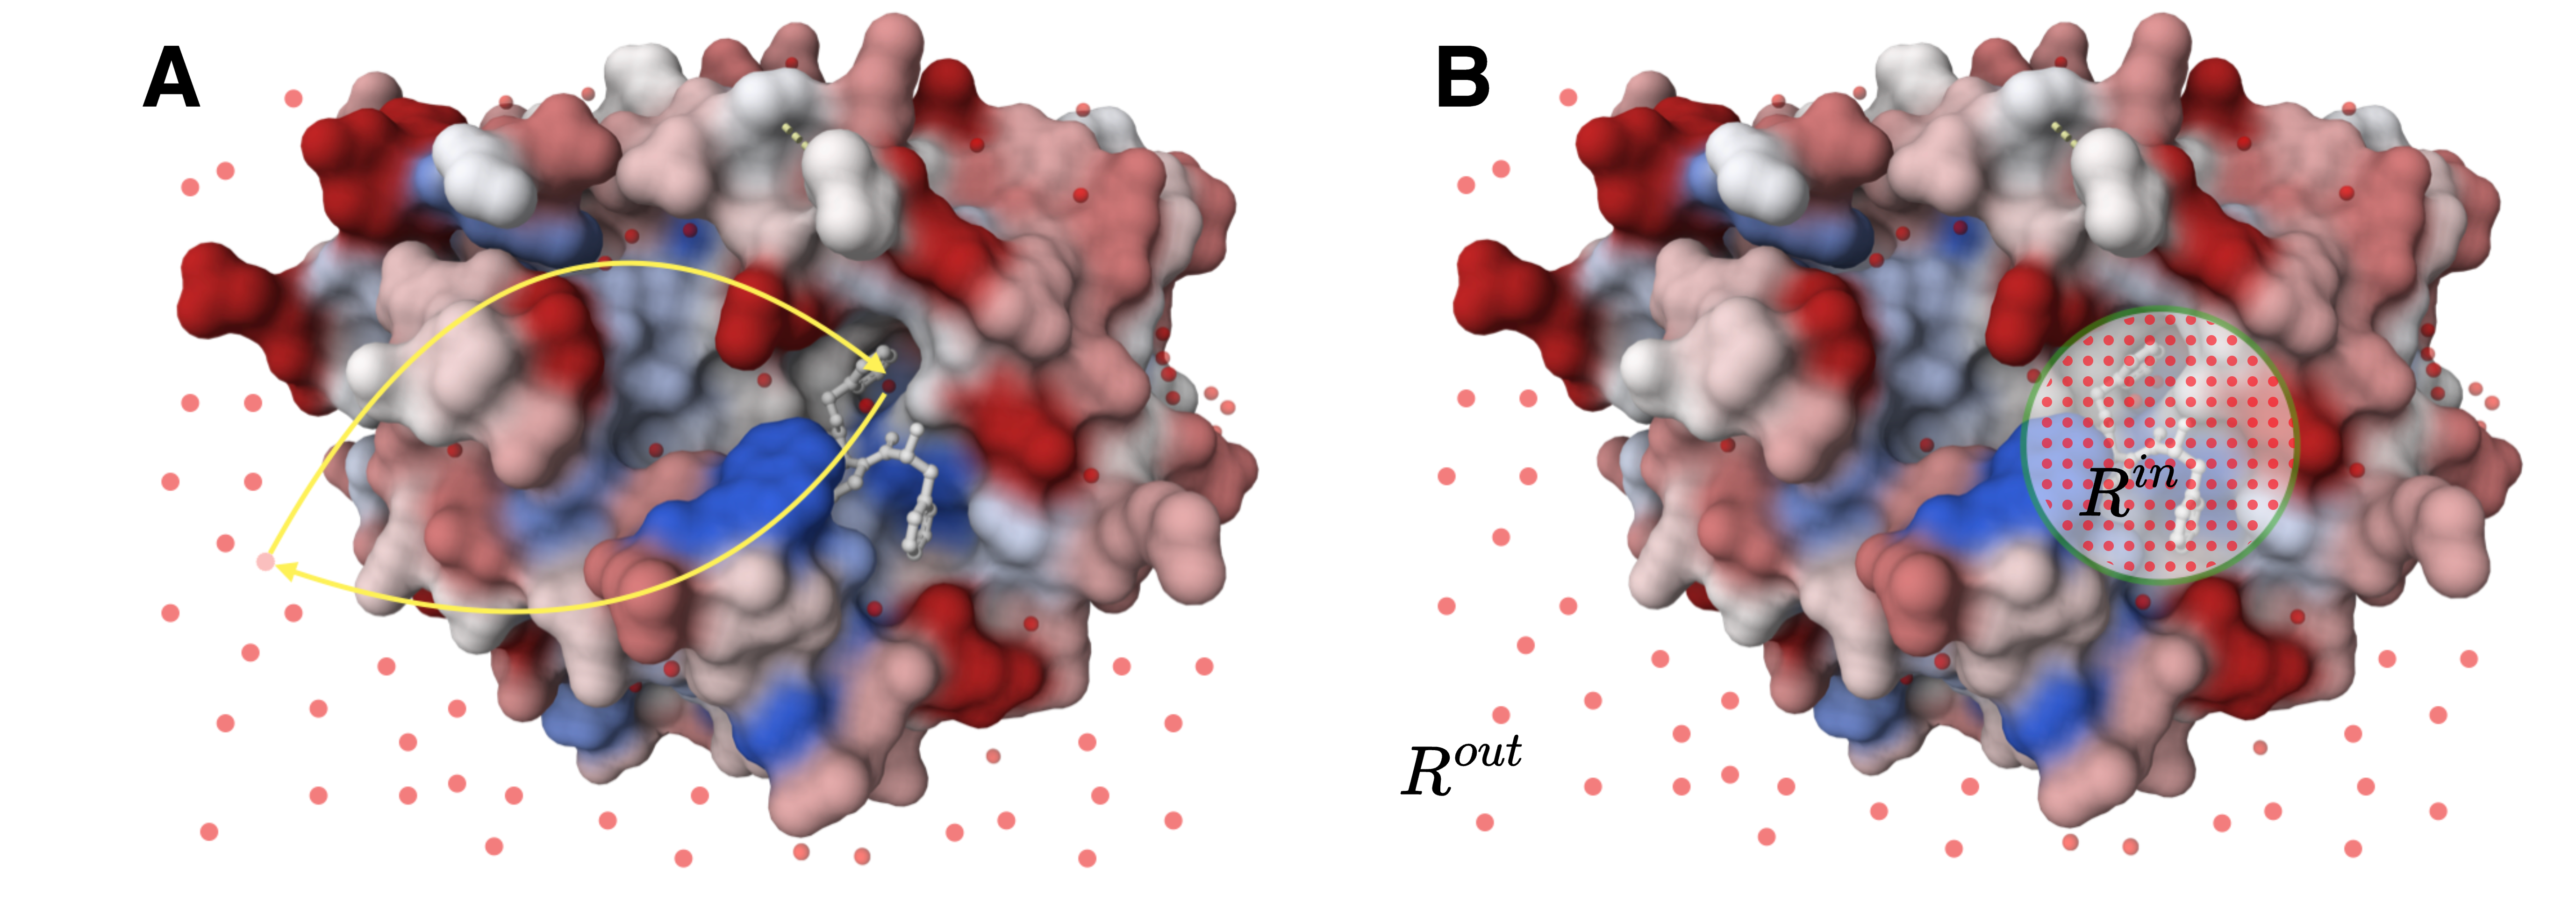
\includegraphics[width=0.9\textwidth]{figures/SwapMonteCarlo-scheme.png}
  \caption{Schematic Figure for Swap Monte Carlo (SwapMC) Method.
  The figure illustrates the process of moving water molecules in and out of the protein cavity during simulation.}
  \label{fig:scheme}
\end{figure}

\subsection{Detailed Balance in Swap Monte Carlo}
In the Monte Carlo algorithm, the acceptance ratio $A_{S_i, S_j}$ between two states $S_i$ and $S_j$ must satisfy detailed balance:
\begin{equation}\label{eq:acceptance_ratio}
\frac{A_{S_i,S_j}}{A_{S_j,S_i}}=\frac{G_{S_j,S_i} P_{S_j}}{G_{S_i,S_j} P_{S_i}}
\end{equation} \\
\noindent Where $P_{S_j}$ and $P_{S_i}$ represent the equilibrium probabilities of states $S_j$ and $S_i$, respectively. 
The terms $G_{S_i, S_j}$ and $G_{S_j, S_i}$ denote the transition probabilities for the transformation from state $S_i$ to state $S_j$, and vice versa.
As the Metropolis criteria indicated, in simulations, the acceptance ratio $A_{S_i,S_j}$ for the transformation from state $S_i$ to $S_j$, is defined as:
\begin{equation}\label{eq:metropolis}
A_{S_i,S_j}=\min \left\{1, \frac{G_{S_j,S_i} P_{S_j}}{G_{S_i,S_j} P_{S_i}}\right\}
\end{equation} \\
\newline
In the context of Swap Monte Carlo, state $S_i$ represent the water molecule located in position $\mathbf{x}_i$, and state $S_j$ represents the water molecule located in position $\mathbf{x}_j$, where the other atoms remains fixed.
Thus, the equilibrium probabilities $P_{S_i}$ and $P_{S_j}$ followed a Boltzmann distribution in the grand canonical ensemble, expressed as:
\begin{equation}\label{eq:equilibrium_probability}
  \begin{aligned}
  P_{S_i}\left(\mathbf{x}_1, \ldots, \mathbf{x}_i, \ldots\mathbf{x}_n\right) & \propto \frac{e^{n B}}{n!} e^{-\beta U\left(\mathbf{x}_1, \ldots, \mathbf{x}_i,\ldots, \mathbf{x}_n\right)}  \\
  P_{S_j}\left(\mathbf{x}_1, \ldots, \mathbf{x}_j, \ldots\mathbf{x}_n\right) & \propto \frac{e^{n B}}{n!} e^{-\beta U\left(\mathbf{x}_1, \ldots, \mathbf{x}_j,\ldots, \mathbf{x}_n\right)}
  \end{aligned}
\end{equation}
\\
Where $U\left(\mathbf{x}_1, \ldots, \mathbf{x}_i,\ldots, \mathbf{x}_n\right), U\left(\mathbf{x}_1, \ldots, \mathbf{x}_j,\ldots, \mathbf{x}_n\right)$ denotes the potential energy of the states $S_i, S_j$, 
$\beta = \frac{1}{kT}$ is the inverse temperature, $k$ is the Boltzmann constant, and $n$ is the number of particles in the system.
A fundamental relationship emerges from the potential energy difference between two states $S_i$ and $S_j$:
\begin{equation}\label{eq:potential_energy_interaction}
U\left(\mathbf{x}_1, \ldots, \mathbf{x}_j,\ldots, \mathbf{x}_n\right) - U\left(\mathbf{x}_1, \ldots, \mathbf{x}_i,\ldots, \mathbf{x}_n\right) = u_j - u_i
\end{equation}
Where $u_i$ and $u_j$ are the interaction energies of the moved water molecule in states $S_i$ and $S_j$, respectively.
\newline
The transition probability matrix element $G_{S_i, S_j}$ quantifies the likelihood of transitioning from state $S_i$ to state $S_j$. 
Given the statistical independence between molecular deletion and insertion events, 
the composite transition probability necessarily factorizes as:
\begin{equation}\label{eq:transition_probability_decomposition}
G_{S_i, S_j} = g_{S_i}^{(\text{del})} \cdot g_{S_j}^{(\text{ins})}
\end{equation}
Where $g_{S_i}^{(\text{del})}$ and $g_{S_j}^{(\text{ins})}$ represent the respective marginal probabilities for water molecule removal from state $S_i$ and insertion into state $S_j$.
With the previous workflow steps, the deletion probability $g_{S_i}^{(\text{del})}$ is defined as the probability of selecting a water molecule $i$ for deletion from the source region, 
given by Eq.~\ref{eq:selection_probability}, 
and the insertion probability $g_{S_j}^{(\text{ins})}$ is defined as the uniform sampling of the potential insertion sites over the destination region.
Thus, the transformation probability matrix elements $G_{S_i, S_j}$ and $G_{S_j, S_i}$ can be expressed as:
\begin{equation}\label{eq:transition_probability}
  \begin{aligned}
G_{S_i, S_j} &= p_i * \frac{1}{18000} = \frac{e^{u_i}}{\sum^{N^{S_i}_{src}}_k{e^{u_k}}} * \frac{1}{18000} \\
G_{S_j, S_i} &= p_j * \frac{1}{18000} = \frac{e^{u_j}}{\sum^{N^{S_j}_{src}}_k{e^{u_k}}} * \frac{1}{18000}  
  \end{aligned}
\end{equation}
The source region cardinalities $N_{\text{src}}^{S_i}$ and $N_{\text{src}}^{S_j}$ in the transition probability elements $G_{S_i, S_j}$ and $G_{S_j, S_i}$ correspond to distinct spatial domains within the simulation framework, 
as their respective source regions differ between the transformation $S_i \to S_j$ and $S_j \to S_i$.
Assume the position $\mathbf{x}_i$ is within the cavity region $R^{in}$, and the position $\mathbf{x}_j$ is outside the cavity region $R^{out}$.
The source region $N_{\text{src}}^{S_i}$ is defined as the set of water molecules within the cavity region $R^{in}$, 
and the source region $N_{\text{src}}^{S_j}$ is defined as the set of water molecules outside the cavity region $R^{out}$ plus the moved water molecule in position $\textbf{x}_j$. \\
%To formally distinguish these non-overlapping regions, we employ the notation $N_{\text{src}}^{S_i}$ and $N_{\text{src}}^{S_j}$ as domain-specific particle counts.
\newline
By substitute the components in Eq.~\ref{eq:metropolis} with the Eq.~\ref{eq:equilibrium_probability},~\ref{eq:potential_energy_interaction},~\ref{eq:transition_probability},
we obtained the acceptance criterion for the exchange of water molecules in transition $S_i \to S_j$:
\begin{equation}\label{eq:acceptance_criterion}
A_{S_i, S_j} = \min \left\{1, \frac{\sum^{N^{S_i}_{src}}_k{e^{u_k}}}{\sum^{N^{S_j}_{src}}_k{e^{u_k}}} \right\}
\end{equation}
\noindent The acceptance criterion required the calculations on the interaction energies $u_k$ of all water molecules in the source region $N^{S_i}_{src}$ or $N^{S_j}_{src}$,
which can be efficiently performed in parallel on GPUs.
\subsection{Implementation of Swap Monte Carlo in Uni-FEP}
To implement the SwapMC method in the Uni-FEP framework, we have rewritten the non-bonded interaction module in OpenMM to support the efficient calculation of interaction energies for water molecules in the simulation box.
Besides, we have also implemented the interaction energy calculation for the inserted water molecules in the potential insertion sites.
The evaluation of the interaction energy for each of the 18,000 water molecules in the simulated system is performed in parallel on GPUs,
allowing for efficient computation of the acceptance ratio $A_{S_i, S_j}$ for each potential insertion conformation.
The implementation of SwapMC is designed to be compatible with the existing Uni-FEP framework, 
without loss of MD simulation performance.
\YE{We need to add the performance comparison with NPT here.}


\section{Results}
For a robust validation of the Swap Monte Carlo method, 
we conducted a series of tests to evaluate its performance in free energy calculations.
Gregory et.al~\cite{ross2020enhancing} performed a comprehensive evaluation of the GCMC method for water sampling in the RBFE calculations.
The test set in Gregory's work includes 94 ligands in 8 diverse protein-ligand systems.
For each system, the transformation of the ligands in RBFE calculations is related to the water displacement in the protein cavity.
GCMC has been shown to be effective in sampling water molecules in the protein cavity~\cite{ross2015water},
and showed a significant improvement in the accuracy of RBFE calculations compared to the traditional MD simulations for RBFE with water displacement transformation.
In this work, we made a direct comparison of the performance of SwapMC with GCMC in the same test cases.
All tests were performed with the Uni-FEP framework~\YE{TO be cited}.
RBFE simulations were performed with the Uni-FEP framework, 
each replica was run for 5~ns with a time step of 4~fs.
SwapMC was performed every 500 steps (2~ps) during the simulation.

\subsection{Water Sampling in Protein Cavity}
For a more intuitive understanding of the water displacement in the protein cavity, 
we have selected two ligands from the HSP90 protein-ligand system, Ligand 9 and Ligand 7, as shown in Fig.~\ref{fig:hsp90} A.
The transformation of Ligand 9 to Ligand 7 involves the core hopping change of the two ligands,
which results in a subtle water distribution change in the protein cavity.
However, the change of the water distribution in the cavity is hard to be captured by the traditional MD simulations.
Especially for the structures without pre-equilibration, the water molecules in the cavity region are not well sampled.\\
\noindent
In the test, we performed the alchemical transformation of Ligand 9 to Ligand 7.
The water molecules in the cavity region were removed in the input structure of the simulation.
Fig.~\ref{fig:hsp90} B showed changes of the number of contact water molecules\YE{Introduce the definition about the contact water molecules here.} in the cavity region with different replicas during the alchemical transformation.
Within the 5~\textit{ns} simulation for each replica, 
the number of contact water molecules with SwapMC is significantly higher than that without SwapMC.
Ligand 7 has larger number of contact water molecules in the cavity region than Ligand 9,
which is consistent with the ligand structure change.
These results indicate that SwapMC made a more thorough sampling of the water molecules in the cavity region.
And it also captured the subtle change of the water distribution in the cavity region with distinct ligands.
With the SwapMC enabled, the RBFE results for the alchemical transformation of Ligand 9 to Ligand 7 is significantly improved 4.59~\textit{kcal/mol} compared to the results without SwapMC.
\begin{figure}
  \includegraphics[width=0.9\textwidth]{figures/hsp90.png}
  \caption{Water sampling in the HSP90 protein cavity in the presence of a ligand. 
  Panel A shows the two ligands (Ligand 9 and Ligand 7) used in the test.
  Panel B shows the number of contact water molecules in the cavity region during the alchemical transformation of Ligand 9 to Ligand 7.
  Replica 0 denotes the Ligand 9 state, and Replica 23 denotes the Ligand 7 state.
  }
  \label{fig:hsp90}
\end{figure}

\subsection{Performance on RBFE Calculations}

\begin{table}
  \caption{RBFE Results on Water-sets}
  \label{tbl:rbfe_watersets}
  \begin{tabular}{l|lllll}
    \hline
    System      & No Cavity Waters + Without SwapMC & No Cavity Waters + With SwapMC & Cavity Waters + Without SwapMC & Cavity Waters + With SwapMC & GCMC by Gregory et.al \\
    \hline
    brd41   & Entry two   \\
    chk1 & Entry four  \\
    HSP90_kung five  & Entry five  \\
    HSP90_Woodhead & Entry eight \\
    scytalone_dehydratase & Entry nine \\
    Taf12 & Entry ten \\
    Thrombin & Entry eleven \\
    Urokinase & Entry twelve \\
    \hline
  \end{tabular}
\end{table}

\subsection{Performance on ABFE Calculations}


\section{Discussion}

%%%%%%%%%%%%%%%%%%%%%%%%%%%%%%%%%%%%%%%%%%%%%%%%%%%%%%%%%%%%%%%%%%%%%
%% The "Acknowledgement" section can be given in all manuscript
%% classes.  This should be given within the "acknowledgement"
%% environment, which will make the correct section or running title.
%%%%%%%%%%%%%%%%%%%%%%%%%%%%%%%%%%%%%%%%%%%%%%%%%%%%%%%%%%%%%%%%%%%%%
\begin{acknowledgement}

Please use ``The authors thank \ldots'' rather than ``The
authors would like to thank \ldots''.

The author thanks Mats Dahlgren for version one of \textsf{achemso},
and Donald Arseneau for the code taken from \textsf{cite} to move
citations after punctuation. Many users have provided feedback on the
class, which is reflected in all of the different demonstrations
shown in this document.

\end{acknowledgement}

%%%%%%%%%%%%%%%%%%%%%%%%%%%%%%%%%%%%%%%%%%%%%%%%%%%%%%%%%%%%%%%%%%%%%
%% The same is true for Supporting Information, which should use the
%% suppinfo environment.
%%%%%%%%%%%%%%%%%%%%%%%%%%%%%%%%%%%%%%%%%%%%%%%%%%%%%%%%%%%%%%%%%%%%%
\begin{suppinfo}

This will usually read something like: ``Experimental procedures and
characterization data for all new compounds. The class will
automatically add a sentence pointing to the information on-line:

\end{suppinfo}

%%%%%%%%%%%%%%%%%%%%%%%%%%%%%%%%%%%%%%%%%%%%%%%%%%%%%%%%%%%%%%%%%%%%%
%% The appropriate \bibliography command should be placed here.
%% Notice that the class file automatically sets \bibliographystyle
%% and also names the section correctly.
%%%%%%%%%%%%%%%%%%%%%%%%%%%%%%%%%%%%%%%%%%%%%%%%%%%%%%%%%%%%%%%%%%%%%
\bibliography{ref, common_ref}

\end{document}